
% \begin{frame}
%  \fontsize{8pt}{10}\selectfont
%   \begin{block}{Randomized SVD Algorithm\footnotemark}\pause
% Given an $m\times n$ matrix $\bs{A}$, a target number $k$ of singular 
% vectors, and an exponent $q$ (say, $q=1$ or $q=2$), this procedure computes an 
% approximate rank-$2k$ factorization $\bs{U}\bs{\Sigma}\bs{V}^*$, where $\bs{U}$ 
% and $\bs{V}$ are 
% orthonormal, and $\bs{\Sigma}$ is nonnegative and diagonal.\\[.2cm]
% \textbf{Stage A:}
% \begin{enumerate}
%   \item Generate an $n\times 2k$ Gaussian test matrix $\bs{\Omega}$.
%   \item Form $\bs{Y}_0 = \bs{A}\bs{\Omega}$ and compute its QR factorization 
% $\bs{Y}_0 = \bs{Q}_0\bs{R}_0$
%   \item \textbf{for} $j = 1, 2, \dots, q$\\
%   \hspace{.4cm} Form $\bs{\widetilde{Y}}_j = \bs{A}^*\bs{Q}_{j-1}$ and compute 
% its QR factorization $\bs{\widetilde{Y}}_j = \bs{\widetilde{Q}}_j 
% \bs{\widetilde{R}}_j$\\
%   \hspace{.4cm} Form $\bs{Y}_j = \bs{A}\bs{\widetilde{Q}}_j$ and compute its QR 
% factorization $\bs{Y}_j = \bs{Q}_j \bs{R}_j$.\\
%   \textbf{end}
%   \item Let $\bs{Q} = \bs{Q}_q$, so that the columns of $\bs{Q}$ form an 
% orthonormal basis for the range of $\bs{Y}$.
% \end{enumerate}
% \textbf{Stage B:}
% \begin{enumerate}
%   \setcounter{enumi}{4}
%   \item Form $\bs{B} = \bs{Q}^* \bs{A}$
%   \item Compute an SVD of the small matrix: 
%   $\bs{B} = \bs{\widetilde{U}} \bs{\Sigma} \bs{V}^*$
%   \item Set $\bs{U} = \bs{Q}\bs{\widetilde{U}}$.
% \end{enumerate}
%   \footnotetext{ \fontsize{6pt}{10}\selectfont $^1$Halko N, Martinsson P-G 
% and Tropp J A 2011 Finding structure with randomness: probabilistic algorithms 
% for constructing approximate matrix decompositions \emph{SIAM} Rev. \textbf{53} 
% 217--88}
%   \end{block}
% \end{frame}


\subsection{RandSVD}

\begin{frame}[fragile]
\fontsize{8pt}{10}\selectfont
\begin{block}{Randomized SVD\footnotemark}
  \begin{minipage}{.55\textwidth}
    \begin{center}
      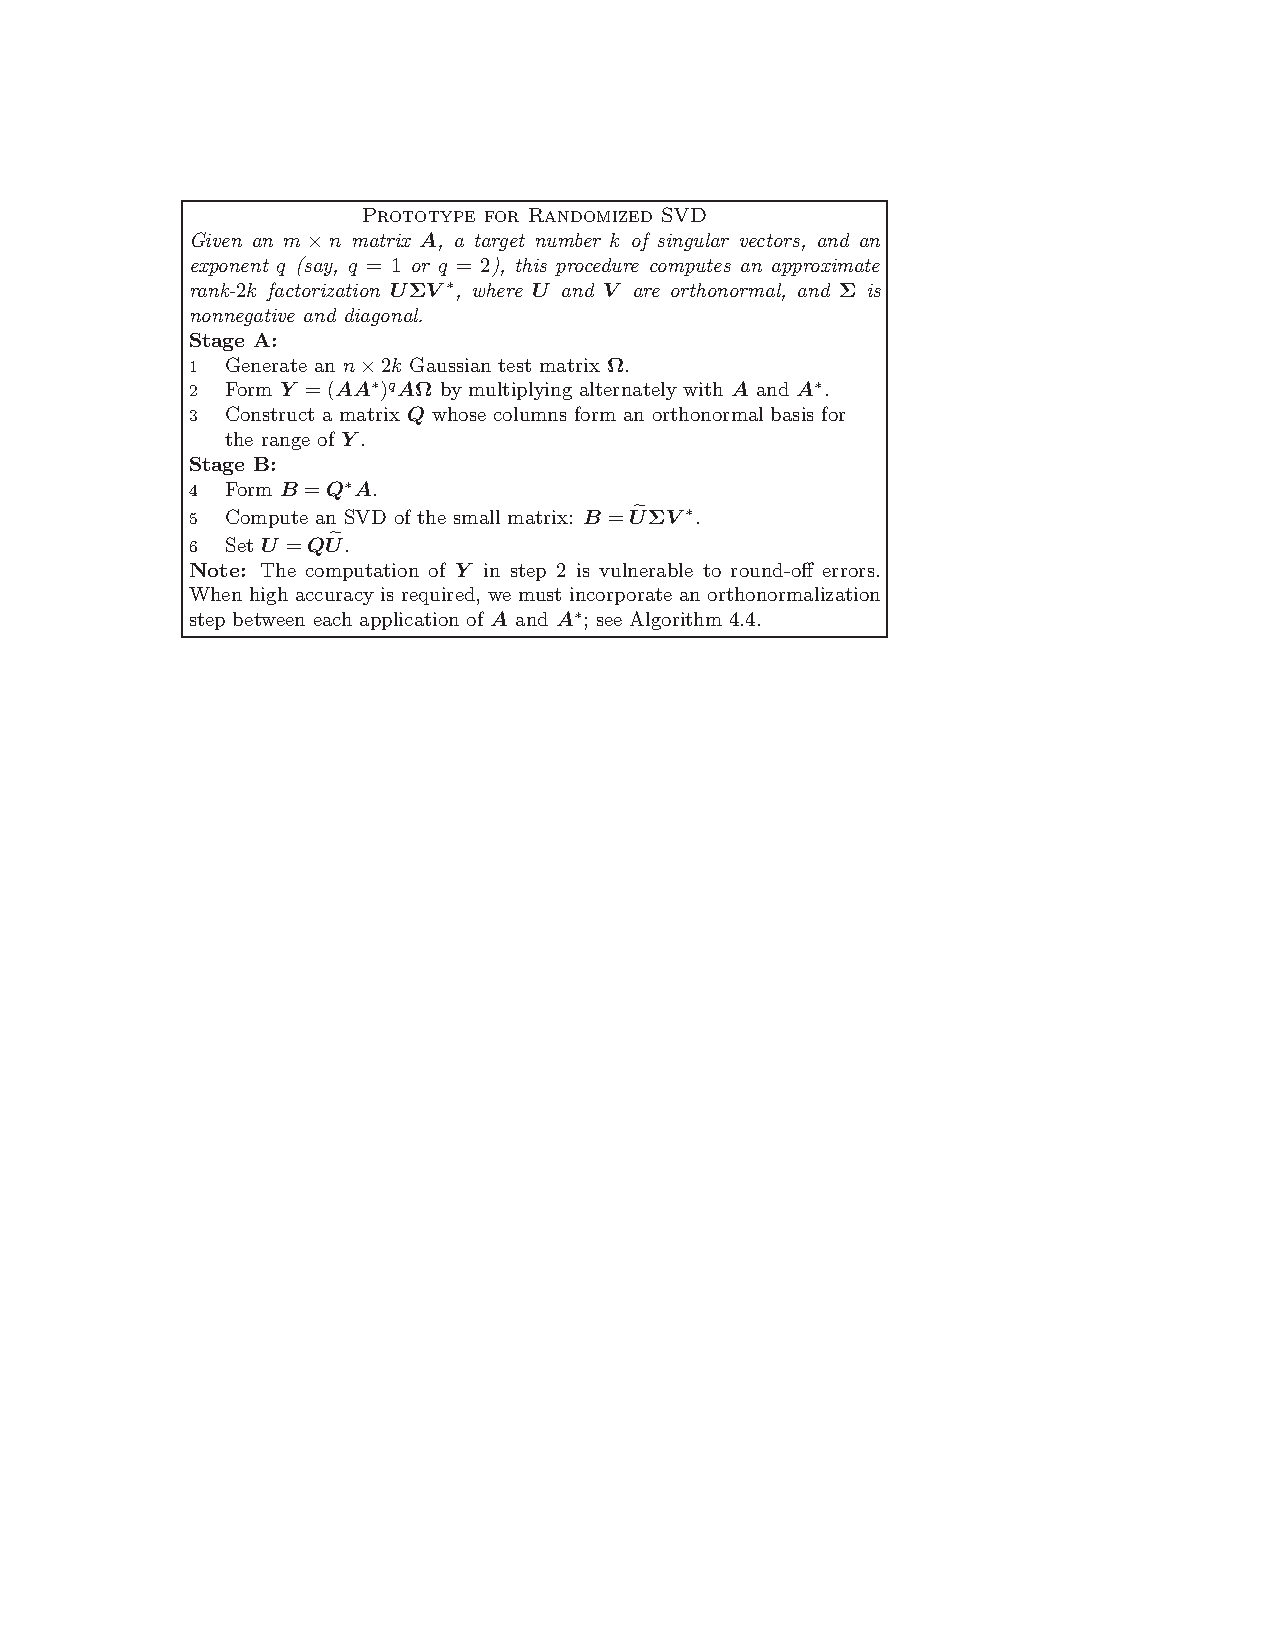
\includegraphics[width=.95\textwidth]{../common/pics/randsvd/randSVDalg}
      \\
      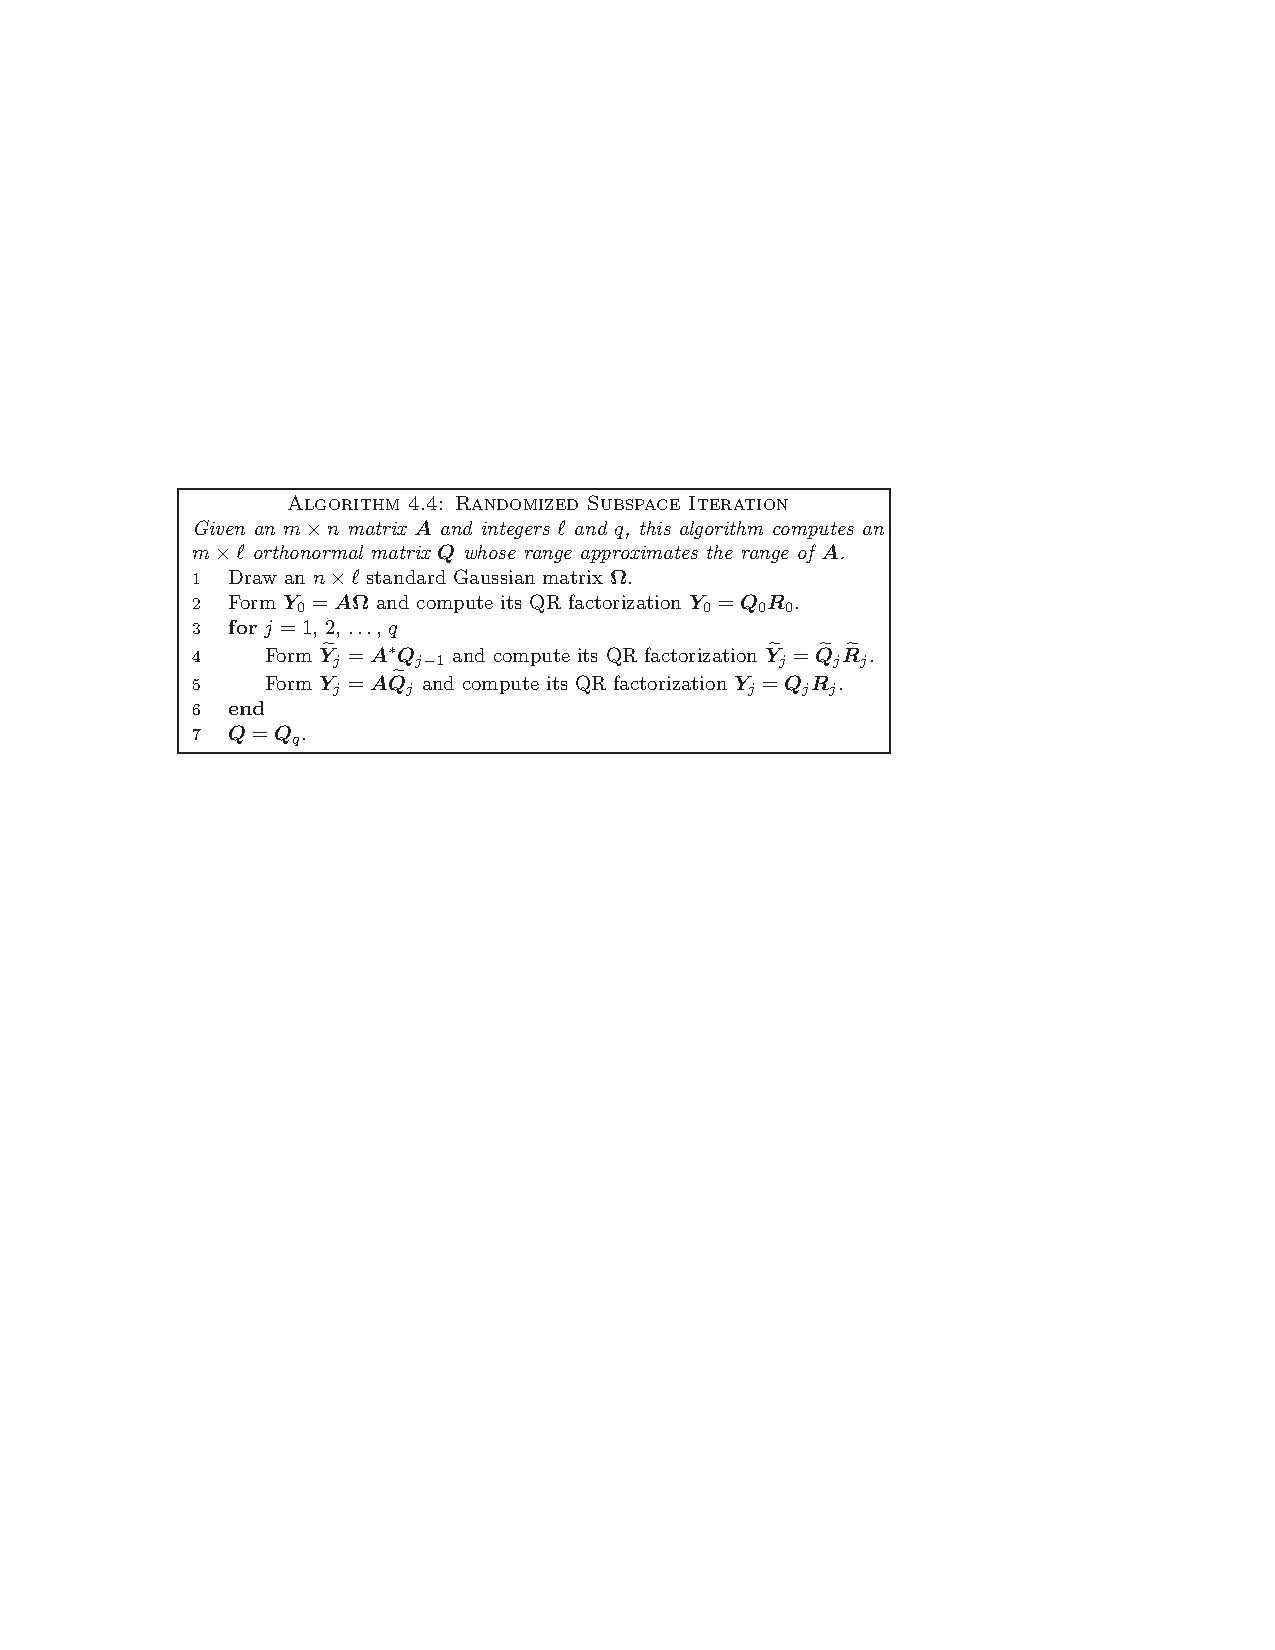
\includegraphics[width=.95\textwidth]{../common/pics/randsvd/randSVDalg4_4}
    \end{center}
  \end{minipage}
%   \hspace{.01cm}
  \begin{minipage}{0.430\textwidth}
\begin{lstlisting}[title=Serial 
R,basicstyle=\tiny,backgroundcolor=\color{grayish} 
,numberstyle=\tiny\color{black},keywordstyle=\color{black},commentstyle=\color{ 
dkgreen},stringstyle=\color{black},escapeinside={(*@}{@*)}]
randSVD <- function(A, k, q=3)
  {
    ## Stage A
    Omega <- (*@ matrix(rnorm(n*2*k),@*) 
            (*@ nrow=n, ncol=2*k) @*)
    Y <- A %*% Omega
    Q <- qr.Q(qr(Y))
    At <- t(A)
    for(i in 1:q)
      {
        Y <- At %*% Q
        Q <- qr.Q(qr(Y))
        Y <- A %*% Q
        Q <- qr.Q(qr(Y))
      }
    
    ## Stage B
    B <- t(Q) %*% A
    U <- La.svd(B)$u
    U <- Q %*% U
    U[, 1:k]
  }
\end{lstlisting} %balance$
\end{minipage}
{\fontsize{6pt}{10}\selectfont $^1$Halko N, Martinsson P-G 
  and Tropp J A 2011 Finding structure with randomness: probabilistic 
algorithms 
  for constructing approximate matrix decompositions \emph{SIAM Rev.} 
\textbf{53} 
  217--88}
\end{block}
\end{frame}


\begin{frame}[fragile]
 \fontsize{8pt}{10}\selectfont
\begin{block}{Randomized SVD}
  \hfill
  \begin{minipage}{0.430\textwidth}
\begin{lstlisting}[title=Serial 
R,basicstyle=\tiny,backgroundcolor=\color{grayish} 
,numberstyle=\tiny\color{black},keywordstyle=\color{black},commentstyle=\color{ 
dkgreen},stringstyle=\color{black},escapeinside={(*@}{@*)}]
randSVD <- function(A, k, q=3)
  {
    ## Stage A
    Omega <- (*@ \textcolor{blue}{matrix(rnorm(n*2*k),} @*) 
         (*@ \textcolor{blue}{ nrow=n, ncol=2*k)} @*)
    Y <- A %*% Omega
    Q <- qr.Q(qr(Y))
    At <- t(A)
    for(i in 1:q)
      {
        Y <- At %*% Q
        Q <- qr.Q(qr(Y))
        Y <- A %*% Q
        Q <- qr.Q(qr(Y))
      }
    
    ## Stage B
    B <- t(Q) %*% A
    U <- La.svd(B)$u
    U <- Q %*% U
    U[, 1:k]
  }
\end{lstlisting} %balance$
  \end{minipage}
  \hfill
  \begin{minipage}{0.430\textwidth}
\begin{lstlisting}[title=Parallel pbdR,basicstyle=\tiny,backgroundcolor=\color{
grayish}, numberstyle=\tiny\color{black},keywordstyle=\color{black},
commentstyle=\color{dkgreen},stringstyle=\color{black},escapeinside={(*@}{@*)}]
randSVD <- function(A, k, q=3)
  {
    ## Stage A
    Omega <- (*@ \textcolor{blue}{ddmatrix("rnorm",} @*)
         (*@ \textcolor{blue}{nrow=n, ncol=2*k)} @*)
    Y <- A %*% Omega
    Q <- qr.Q(qr(Y))
    At <- t(A)      
    for(i in 1:q)
      {
        Y <- At %*% Q   
        Q <- qr.Q(qr(Y))
        Y <- A %*% Q    
        Q <- qr.Q(qr(Y))
      }
    
    ## Stage B
    B <- t(Q) %*% A     
    U <- La.svd(B)$u 
    U <- Q %*% U     
    U[, 1:k]
  }
\end{lstlisting}  % balancing $
  \end{minipage}
\hfill
\end{block}
\end{frame}

\begin{frame}
  \begin{block}{Randomized SVD}
    \begin{center}
      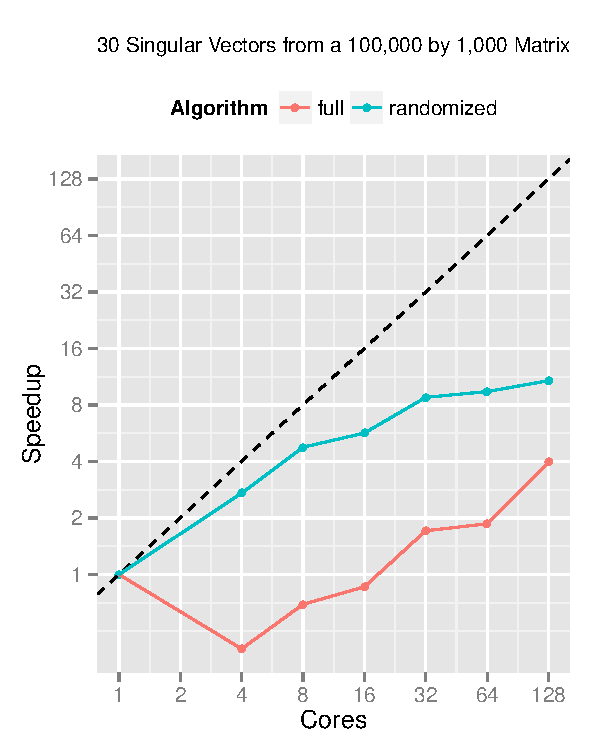
\includegraphics[width=.45\textwidth]{../common/pics/randsvd/randSVDspeedup}
      \hfill
      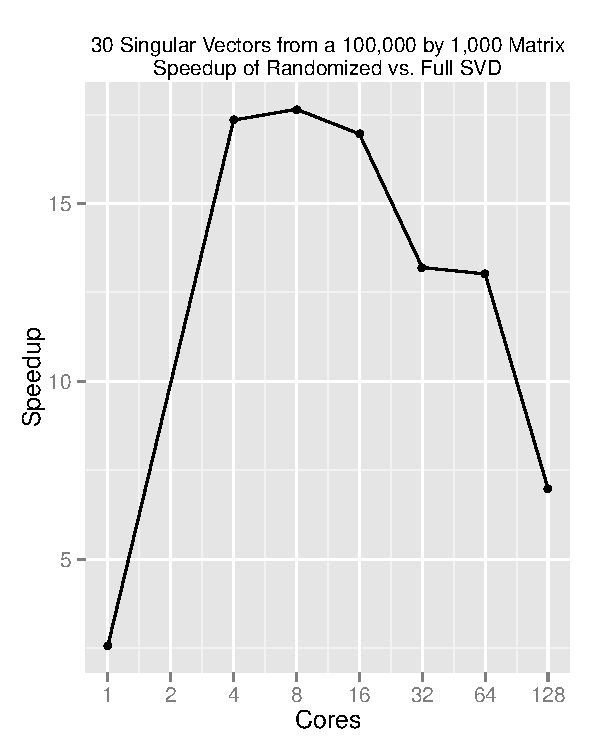
\includegraphics[width=.45\textwidth]{../common/pics/randsvd/randSpeedupSVD}
    \end{center}
  \end{block}
\end{frame}